\chapter{Applicazioni}\label{applicazioni}
\section{Measured Boot, Secure Boot e Trusted Boot}\label{sec:boot_types}

Nel paragrafo 1.2 Root of Trust si introduce il concetto di Root of Trust e le sue funzioni principali; tra questi ritroviamo il boot sicuro, descritto come l’instaurazione di una catena di fiducia necessaria per garantire un processo di avvio sicuro, garantire che il sistema sia in uno stato previsto (integrità della piattaforma) e rilevare eventuale codice manomesso. In altre parole, le \acrshort{rot} permettono a una piattaforma di dimostrare che è un ambiente affidabile.

All'accensione di un computer, il chip UEFI (che ha sostituito il tradizionale BIOS) viene eseguito per primo, ancora prima che qualsiasi altro componente entri in funzione. Il compito del UEFI è identificare l’hardware presente, configurarne il funzionamento, applicare le impostazioni correnti e determinare il dispositivo da cui eseguire l'avvio. Tuttavia, proprio perché questa fase precede l'attivazione di qualsiasi software di sicurezza e persino il caricamento del sistema operativo, rappresenta un momento vulnerabile in cui un hacker potrebbe iniettare codice malevolo per compromettere l'integrità del sistema. Per questo motivo, garantire che l’avvio della piattaforma avvenga in un ambiente sicuro e con codice affidabile è un requisito fondamentale per la protezione del sistema.

C’è molta confusione riguardo i concetti di Measured, Secured e Trusted boot, in questo capitolo si cerca di fare un po’ di chiarezza sui tre e su cosa li distingue uno dall’altro.

È essenziale tenere a mente che sono tre processi separati e differenti fra loro (soprattutto Measured e Secured). Il processo di avvio sicuro consolidato al momento, prevede che l’ordine di esecuzione delle tre fasi sia Measured Boot - Secure Boot - Trusted Boot. In realtà nessuna fase è obbligatoria, ma questo verrà esplorato più nel dettaglio nelle sezioni seguenti.

\subsection{Measured Boot}\label{subsec:measured_boot}

Il Measured Boot è un componente essenziale dell'architettura \acrshort{tpm} ed è alla base di molti altri meccanismi di sicurezza. Il suo scopo principale è garantire l’integrità dell’ambiente di pre-boot, ovvero la fase iniziale del processo di avvio, prima che il sistema operativo venga caricato. Il firmware e i bootloader del sistema utilizzano il \acrshort{tpm} per registrare e verificare che nessun componente sia stato alterato.

Questo processo si basa su una tecnica chiamata hash chaining, in cui ogni misurazione viene combinata con quella precedente attraverso un'operazione di hash extend (descritta nel capitolo 1.4.2.1). La specifica della piattaforma definisce quali \acrshort{pcr} devono essere utilizzati per ciascun componente del boot, e il primo codice eseguito –- che può essere il boot block del BIOS o l’intero firmware UEFI -– deve essere completamente protetto in scrittura. Questo impedisce a un attaccante di alterare il processo e registrare misurazioni false, preservando così l’attendibilità del sistema.

\begin{figure}[htbp]
    \centering
        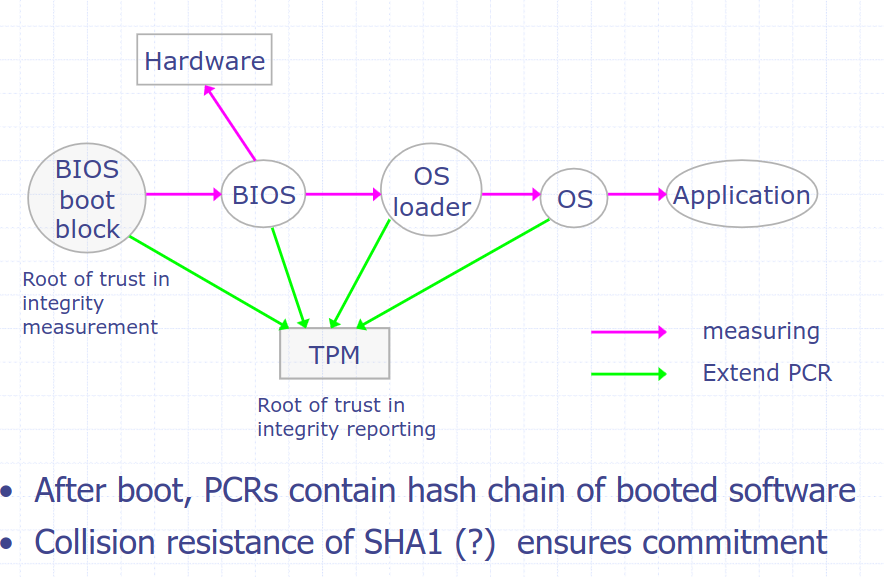
\includegraphics[width=0.77\textwidth]{figures/architettura-tcg.png}
    \caption{Slide dal corso sull’architettura \acrshort{tcg} della Stanford University.}
    \label{fig:architettura-tcg}
\end{figure}

Come conseguenza a questo processo, i \acrshort{pcr} conterranno la “hash-chain” calcolata su tutto il firmware, software e configurazioni della piattaforma.

UEFI inoltre abilita il Measured Boot a compiere un’operazione chiamata Remote Attestation che confronta le informazioni memorizzate nel \acrshort{tpm} con una versione sicura archiviata su un computer esterno, come un server aziendale o un servizio come Microsoft Endpoint Manager (InTune). Se i valori coincidono, significa che il \acrshort{tpm} non è stato alterato.

Nonostante la sua efficacia, Measured Boot is raramente utilizzato. La sua implementazione richiede un'infrastruttura complessa, con server di riferimento sicuri per la verifica, aumentando i costi e la difficoltà di gestione. Inoltre, la scarsa standardizzazione nell’uso dei \acrshort{pcr} e la compatibilità limitata con alcuni dispositivi e sistemi operativi ne ostacolano l'adozione. Soluzioni più semplici come Secure Boot e Trusted Boot sono spesso ritenute sufficienti, mentre Measured Boot resta principalmente una misura di sicurezza per ambienti ad alto rischio, come istituzioni governative o grandi enti finanziari.

\subsection{Secure Boot}\label{subsec:secure_boot}

Measured Boot conferma che il firmware e software non siano stati compromessi, quindi lo possiamo intuire come un controllo logico del codice e delle configurazioni della piattaforma. Il Secure Boot è invece un controllo hardware che assicura che il bootloader non sia stato manomesso. Fa parte dell'UEFI, un insieme di routine che forniscono le funzionalità di base per l'avvio del computer.

Secure Boot entra in gioco subito dopo l’avvio, o quando Measured Boot ha confermato con successo l'integrità del sistema se quest’ultimo è attivo. In pratica, verifica che tutto il codice eseguito prima del caricamento del sistema operativo sia affidabile: lo garantisce controllando che il firmware sia firmato digitalmente, riducendo il rischio di rootkit.

Solo il codice approvato dal produttore o dall'utente può essere eseguito. Se il bootloader o un altro componente non è firmato correttamente o non è riconosciuto dal produttore della scheda madre, come nel caso di software di terze parti, l'avvio viene impedito. Perseguendo gli obiettivi di una Root of Trust, Secure Boot permette di creare un percorso sicuro e affidabile che parte dall'UEFI e prosegue fino al kernel del sistema operativo.

È importante notare che, sebbene Secure Boot e Measured Boot condividano l'obiettivo di proteggere il sistema, differiscono nel modo in cui lo fanno. Secure Boot si limita a verificare la firma digitale del bootloader, mentre Measured Boot esegue un controllo più approfondito, registrando l'intero stato del software di avvio in modo verificabile successivamente. Tuttavia, il \acrshort{tpm} non impedisce direttamente l'avvio se rileva codice manomesso, il suo ruolo è solo quello di registrare i cambiamenti, lasciando ad altri meccanismi di sicurezza la decisione su come reagire. Solo Secure Boot ha la competenza di arrestare la sequenza d’avvio.

\subsection{Trusted Boot}\label{subsec:trusted_boot}

Se Secure Boot non rileva alcun problema e il processo di avvio prosegue, allora si attiva Trusted Boot, che effettua un ulteriore controllo per verificare che il bootloader, il kernel e altri componenti di basso livello non siano stati alterati dopo l’ultimo spegnimento del sistema. Trusted Boot è un meccanismo software che confronta il codice di avvio con i dati memorizzati nel \acrshort{tpm} durante l'ultimo arresto del sistema. Durante il Secure Boot il codice del \acrshort{so} non è disponibile, perché non è ancora stato caricato, mentre il Trusted Boot permette di verificare anche questi file.

Questa fase continua la chain of trust: il bootloader (verificato dal Secure Boot) verifica la firma digitale del kernel, mentre il kernel a sua volta controlla ogni altro componente dell’ambiente pre-boot del sistema operativo - inclusi i driver e i file di avvio. Come il Secure Boot, Trusted Boot è in grado di bloccare l’avvio di firmware o software modificato.

Per il \acrshort{tcg} il Trusted Boot è parte integrante della specifica, ma le implementazioni sono lasciate ai singoli sistemi operativi. Per le macchine che montano \acrshort{cpu} Intel-based il progetto di riferimento è tboot, un modulo open source che fa uso della tecnologia Intel Trusted Execution Technology. Per le piattaforme \acrshort{amd} il concetto è ripreso dalla tecnologia \acrshort{amd} Platform Security Processor. Una nota: l’azienda produttrice di \acrshort{amd} PSP ha rifiutato di rendere open source il progetto, suscitando critiche e accuse relative a possibili backdoor o meccanismi simili.

\section{Esempio di Measured Boot con Attestazione Remota}\label{sec:esempio_measured_boot}

Il sistema operativo Windows dalla versione 10 in poi, implementa tutti e tre i moduli Measure Boot (se il \acrshort{tpm} 2.0 è presente), Secure Boot e Trusted Boot -- sebbene siano tutti disattivabili dall’utente.

La minaccia principale da cui intende proteggere il \acrshort{pc} sono i rootkit, un tipo di malware sofisticato che opera in modalità kernel, utilizzando gli stessi privilegi del sistema operativo. Poiché i rootkit hanno gli stessi diritti del sistema operativo e si avviano prima di esso, possono nascondersi completamente agli occhi del \acrshort{so} o software anti-virus.

Nell’immagine di seguito (Figura 7) si osserva uno schema della chain of trust quando tutte e tre le fasi sono attive.

\begin{figure}[htbp]
    \centering
        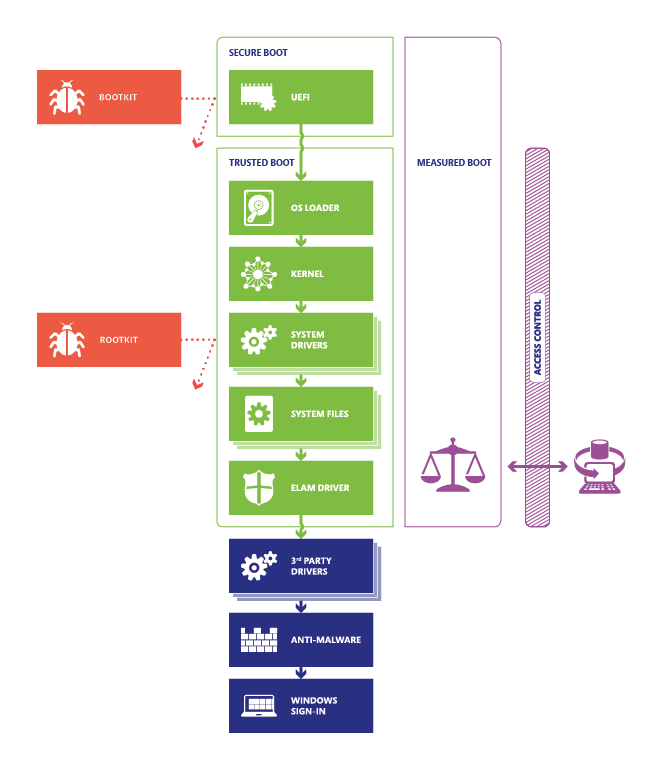
\includegraphics[width=0.8\textwidth]{figures/chain-of-trust.png}
    \caption{Processo di startup del sistema operativo Windows.
    }\label{fig:chain-of-trust}
\end{figure}

Un’aggiunta specifica dell’implementazione Microsoft è \acrfull{elam}, un modulo che interviene dopo la verifica del kernel da parte di Trusted Boot. Questo modulo testa i driver di avvio per verificare che tra questi non si nasconda del malware.

Measured Boot svolge il suo ruolo e le sue funzioni tradizionali come descritte nel capitolo 5.1.1, con la particolarità che necessita di una connessione ad un server di attestazione remoto per confermare le misurazioni \acrshort{tpm} ed i certificati sulla macchina locale.

In particolare l’implementazione di Windows segue questi passi:
\begin{itemize}
    \item Il firmware UEFI del \acrshort{pc} memorizza nel \acrshort{tpm} un hash del firmware, del bootloader, dei driver di avvio e di tutto ciò che viene caricato prima dell'app anti-malware.
    \item Al termine del processo di avvio, Windows avvia il client di attestazione remota. Il server invia al client una chiave unica.
    \item Il \acrshort{tpm} utilizza la chiave per firmare digitalmente il log registrato dall'UEFI.
    \item Il client invia il log al server, eventualmente insieme ad altre informazioni di sicurezza. A seconda dell'implementazione e della configurazione, il server può ora determinare se il client è sicuro.
\end{itemize}

\begin{figure}[htbp]
    \centering
    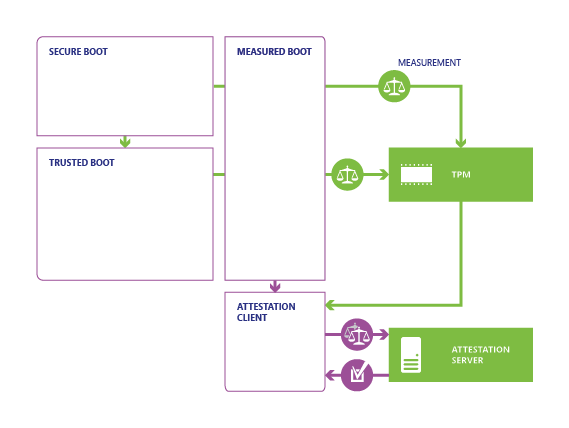
\includegraphics[width=0.5\textwidth]{figures/boot.png} 
    \caption{Attestazione Remota per il Measured Boot}\label{fig:remote_boot}
\end{figure}

Definiamo cosa si intende per Attestazione Remota (o Remote Attestation - RA): l'attestazione remota è un processo in cui una piattaforma fornisce prove verificabili sul suo stato di integrità a un verificatore remoto. Questo meccanismo consente di determinare se un sistema è sicuro senza la necessità di un'autorità di certificazione esterna, perché il verificatore può anche essere un server su cui sono depositati certificati o signatures digitali.

\section{BitLocker}\label{sec:bitlocker}

BitLocker è la funzionalità di crittografia completa del disco di Microsoft per Windows, introdotta in Windows Vista, progettata per proteggere i dati in caso di perdita, furto o smaltimento inappropriato del dispositivo. A partire da Windows 10 Versione 1511, BitLocker utilizza l'algoritmo di crittografia \acrshort{aes}-\acrshort{xts} per crittografare l'intero volume. Di default la chiave è di 128 bit ma è possibile usarne anche da 256 bit.

Il funzionamento di BitLocker si basa su una gerarchia di chiavi crittografiche. Alla base vi è la Full Volume Encryption Key (\acrshort{fvek}), utilizzata per crittografare l'intero disco e viene memorizzata nei metadati del disco in forma cifrata. La Volume Master Key (\acrshort{vmk}) protegge la \acrshort{fvek} ed è a sua volta crittografata tramite uno o più protector (protettori di chiave), come il Trusted Platform Module (\acrshort{tpm}), un \acrshort{pin} o una chiave USB.

Questo sistema a più livelli permette di cambiare le chiavi superiori senza dover decifrare e ri-cifrare l'intero volume, aumentando la flessibilità e la sicurezza del sistema. Quando una KPs è compromessa, vengono create nuove KPs e una nuova chiave principale del volume (\acrshort{vmk}), e la vecchia chiave di crittografia del volume completo (\acrshort{fvek}) viene crittografata con la nuova \acrshort{vmk}. In questo modo, anche se un attaccante ottiene la vecchia KPs, non può decifrare la \acrshort{fvek}.

\subsection{Processo di boot}\label{subsec:processo_de_boot}

BitLocker è generalmente integrato nel bootloader di Windows e viene eseguito prima della selezione del sistema operativo. Ma come fa Windows a riconoscere che il disco è crittografato?

Innanzitutto, BitLocker memorizza le informazioni relative alla crittografia del disco, inclusa l'eventuale presenza e posizione di una chiave. Durante il processo di avvio, diversi componenti del sistema, come il BIOS o UEFI, calcolano l'hash del proprio firmware e della configurazione, inviando poi tale valore al \acrshort{tpm}. Successivamente, il bootloader analizza i metadati del disco per determinare se sia crittografato. Se tutti i controlli sui file di avvio vengono superati, il sistema procede con l’esecuzione del kernel.

A questo punto, il kernel del sistema operativo inizializza le risorse necessarie e rileva l’unità crittografata. Tramite il \acrshort{tpm}, richiede l’accesso alla \acrshort{vmk}, necessaria per decrittografare la \acrshort{fvek} che poi viene utilizzata per decrittografare il contenuto del disco.

Infine, il kernel continua il processo di avvio decifrando ulteriori sezioni dell’unità man mano che diventano necessarie. In presenza del Trusted Boot, il kernel si occuperà anche di calcolare l’hash di alcuni file d’avvio e li invierà ai \acrshort{pcr}.

\subsection{Modalità di utilizzo}\label{subsec:modalita_di_utilizzo}

BitLocker offre tre modalità operative, delle quali le prime due richiedono la presenza di un modulo hardware per la crittografia, il \acrshort{tpm} versione 1.2 o successiva, e un firmware UEFI compatibile:
\begin{itemize}
    \item \textbf{Modalità Trasparente}: Questa modalità sfrutta le capacità del \acrshort{tpm} 1.2 per garantire un'esperienza utente senza interruzioni. La chiave di crittografia del disco viene memorizzata in forma crittografata all'interno del \acrshort{tpm}. Il caricatore del sistema operativo può accedere a questa chiave solo se i file di avvio risultano integri.
    \item \textbf{Modalità di Autenticazione Utente}: In questa modalità, l'utente è tenuto a inserire una chiave di autenticazione nell'ambiente pre-boot per poter avviare il sistema operativo. Sono supportati due metodi di autenticazione, tramite \acrshort{pin} (definito dall’utente) o chiave USB contenente la chiave di avvio necessaria per l'accesso al sistema.
    \item \textbf{Modalità Chiave USB (senza \acrshort{tpm})}: Questa modalità consente l'uso di BitLocker su sistemi privi di \acrshort{tpm}. È importante notare che questa modalità richiede che il BIOS o il firmware UEFI del sistema supporti la lettura dei dispositivi USB durante il processo di avvio. Inoltre, per il corretto funzionamento di BitLocker in questa configurazione, è necessario che il disco rigido sia formattato in almeno due volumi NTFS, uno di sistema e uno di avvio.
\end{itemize}

È fondamentale sottolineare che, nelle versioni client (ovvero non destinate ad un pubblico esperto) di Windows, solo il volume del sistema operativo può essere crittografato utilizzando BitLocker. Per la crittografia di dati sensibili in tempo reale su partizioni NTFS, si raccomanda l'uso del Encrypted File System (EFS), che può essere utilizzato in combinazione con BitLocker per una protezione aggiuntiva.

\subsection{Chiavi}\label{subsec:chiavi}

\textbf{STARTUP KEY}: L'amministratore del \acrshort{pc} crea una chiave di avvio durante l'inizializzazione di BitLocker. La chiave viene memorizzata su qualsiasi dispositivo di archiviazione come una chiavetta USB collegabile, e l'utente deve inserire tale dispositivo nel computer ogni volta che il computer viene avviato o riprende dallo stato di ibernazione. Mentre la chiavetta USB contenente la chiave di avvio deve essere collegata al computer dall'accensione fino al completamento dell'avvio, dovrebbe essere rimossa dopo il caricamento di Windows.

\textbf{RECOVERY KEY}: La chiave di ripristino può essere creata e salvata su una chiavetta USB durante la configurazione di BitLocker. Se il computer entra in modalità di ripristino, verrà richiesto all'utente di inserire la chiave di ripristino nel computer.

\textbf{CLEAR KEY}: se la verifica dell'integrità del sistema è disabilitata, la chiave principale di BitLocker è accessibile senza necessità di autenticazione. La sospensione di BitLocker cripta la chiave principale con una clear key, che è una chiave non protetta sul disco. Questo consente di apportare modifiche al sistema senza dover decifrare e ri-cifrare l'intero disco. Dopo le modifiche, quando BitLocker viene riattivato, quest'ultima sigilla nuovamente la chiave di crittografia con i nuovi valori dei componenti e cancella la clear key. Sebbene si tratti di una casistica che ricade nella manutenzione o quando si effettua un backup, dunque si tende ad eseguire queste operazioni in un ambiente sicuro e con tutte le precauzioni del caso, questa pseudo-esposizione della \acrshort{fvek} risulta una forte vulnerabilità in caso di attaccanti preparati.

\subsection{Critiche}\label{subsec:critiche}

Durante alcune operazioni di backup e ripristino, BitLocker non cifra i volumi finché l’utility di backup di Windows non riceve conferma dall’utente. Di conseguenza, i dati rimangono disponibili in chiaro durante la finestra temporale tra la preparazione del backup e la conferma. Questo consentirebbe ad un attaccante con accesso fisico di interrompere la decifratura automatica del disco durante un riavvio della macchina ed estrarre le chiavi. Sebbene si tratti di una casistica relativamente rara, Microsoft ha dichiarato che tale attacco è possibile solo quando BitLocker è configurato in modalità \acrshort{tpm}-only, che è la modalità predefinita. La configurazione di BitLocker con \acrshort{tpm}+\acrshort{pin}, invece, non è immediata e potrebbe risultare complessa per gli utenti meno esperti.

Nonostante Microsoft abbia negato la presenza di backdoor, la tecnologia supporta una "chiave di recupero" che potrebbe permettere l'accesso ai dati senza il consenso dell'utente, se questa chiave finisse nelle mani sbagliate.

Inoltre il fatto che il kernel venga caricato prima della vera e propria decifratura può rappresentare un ulteriore punto di vulnerabilità ad attacchi sofisticati che riescono a nascondersi e intercettare le chiavi crittografiche.

\subsection{Nota su \texorpdfstring{\acrshort{xts}}{XTS}}\label{subsec:nota_su_xts}

\acrshort{xts} è una soluzione di compromesso tra efficienza e sicurezza per la cifratura dei dischi, ma presenta limiti significativi che lo rendono inadatto come standard universale o per un utilizzo generalizzato e diffuso. La sua protezione è efficace solo quando il dispositivo è spento o bloccato, mentre a sistema acceso i dati rimangono accessibili, riducendo la sicurezza complessiva.

In un documento IEEE del 2007 viene segnalato che \acrshort{xts} è suscettibile alla manipolazione dei dati, poiché non prevede meccanismi di autenticazione: qualsiasi testo cifrato, anche se alterato da un attaccante, verrà comunque decifrato in un testo in chiaro senza alcun sistema integrato per rilevare modifiche o manomissioni. Per questo motivo, le applicazioni che richiedono una protezione più robusta devono adottare misure aggiuntive per verificare l’integrità dei dati e prevenire attacchi come la sostituzione di settori con versioni precedenti o la modifica di eseguibili.

Ulteriori critiche relative alla standardizzazione emergono anche da commenti pubblici su \acrshort{xts}-\acrshort{aes} richiesti dal NIST, successivi al documento IEEE del 2007.

Altri limiti di \acrshort{xts}-\acrshort{aes}: la sua struttura utilizza blocchi \acrshort{aes} da 16 byte, il che permette la manipolazione dei dati cifrati. Inoltre, presenta debolezze matematiche che consentono di recuperare il tweak principale in unità di dati grandi (ad esempio, su hard disk di grandi dimensioni). Inoltre, è vulnerabile ai timing attack.

Dal punto di vista tecnico, il riutilizzo delle chiavi su più blocchi e l'assenza di collegamento tra blocchi cifrati successivi espongono \acrshort{xts} a vulnerabilità come attacchi "taglia e incolla" e manipolazioni simili a quelle della modalità ECB, che può rivelare pattern nel testo cifrato. Di conseguenza, \acrshort{xts} è una soluzione di compromesso, adatta alla cifratura dei dischi, ma con limitazioni crittografiche rilevanti. Per mitigare queste debolezze, è fondamentale che le applicazioni implementino misure come l'uso di ridondanza nei testi in chiaro e il mantenimento di checksum per i dati, adottato nei file system come ZFS o Btrfs.

Per queste ragioni, \acrshort{xts} è considerabile al limite del compromesso accettabile. Alla luce delle criticità evidenziate da esperti nel settore, se \acrshort{xts}-\acrshort{aes} non è considerato idoneo per essere adottato come standard crittografico allora anche, la sua implementazione in sistemi ampiamente diffusi, come Windows, risulterebbe altamente sconsigliata. Questo è particolarmente rilevante considerando che la maggior parte degli utenti di tali sistemi non possiede le competenze necessarie per utilizzare consapevolmente questo strumento, aumentando così il rischio di un impiego non sicuro.

\subsection{Considerazioni}\label{subsec:considerazioni}

Nonostante le criticità progettuali, BitLocker, risi presenta come una soluzione adeguata per utenti non esperti e con esigenze di sicurezza limitate. BitLocker si avvale, infatti, di ulteriori misure di protezione, quali la verifica dell'integrità del bootloader e del kernel del sistema operativo. Pertanto, è raro che si verifichino le vulnerabilità discusse nelle sezioni precedenti, o, qualora si manifestino, sono generalmente presenti livelli di protezione superiori.

\subsection{Attacco BUS Sniff a BitLocker}\label{subsec:attacco_bus_sniff}

Un attacco recentemente dimostrato su un laptop ha consentito di estrarre la chiave di decrittazione di BitLocker in soli 43 secondi, utilizzando un Raspberry Pi Pico a basso costo. Questo exploit ha permesso di accedere e persino modificare i dati crittografati, mettendo in evidenza una vulnerabilità significativa.

Questo tipo di attacco non è una novità, in quanto Microsoft ne è a conoscenza e lo documenta nella sezione dedicata alle contromisure di BitLocker. L'azienda afferma che un attacco di questa natura richiede competenze avanzate, strumenti sofisticati e un accesso fisico prolungato. Ciò nonostante, la recente dimostrazione ha mostrato che, con una preparazione minima, è possibile eseguire l'attacco in meno di 50 secondi, utilizzando dispositivi economici e facilmente reperibili.

Durante l’avvio del sistema, i diversi componenti, come il BIOS/UEFI, eseguono una misurazione dell’integrità (come descritto nel capitolo 5.1). Se le misurazioni correnti corrispondono agli hash nei \acrshort{pcr}, allora il \acrshort{tpm} sblocca la chiave di BitLocker e la trasmette al processore.

Esiste, tuttavia, una vulnerabilità critica: la comunicazione tra il processore e il \acrshort{tpm} non è crittografata, e la chiave viene trasmessa in chiaro. Intercettando il traffico sul bus LPC (Low Pin Count), utilizzato da alcuni laptop per collegare il \acrshort{tpm} alla \acrshort{cpu}, è possibile estrarre la chiave di decrittazione. Per dimostrare tale vulnerabilità, è stato sviluppato un plugin per analizzatore logico, capace di monitorare il traffico su questo bus e di catturare la chiave di BitLocker.

Un attaccante, utilizzando un dispositivo basato su Raspberry Pi Pico, è riuscito a intercettare la comunicazione tra il \acrshort{tpm} e la \acrshort{cpu}, catturando la \acrshort{vmk} all'avvio del sistema. Con questa chiave, è possibile decrittografare l'SSD protetto da BitLocker usando un altra macchina con uno strumento come Dislocker, ottenendo accesso ai dati. Sebbene lo strumento sia stato progettato per un tipo specifico di laptop, non è inusuale trovare computer con un accesso simile ai pin del \acrshort{tpm}.

Questa dimostrazione evidenzia come, nonostante le misure di sicurezza di BitLocker, la protezione della chiave di decrittazione risulta vulnerabile se la comunicazione con il \acrshort{tpm} non è adeguatamente protetta.

\subsubsection{Mitigare l’attacco}\label{subsubsec:mitigare_attacco}

Alcune \acrshort{cpu} moderne sono dotate di f\acrshort{tpm} rendendo difficile intercettare il traffico sul bus -- anche se gli f\acrshort{tpm} non sono generalmente più sicuri dei d\acrshort{tpm}. Tuttavia, molti laptop aziendali continuano a utilizzare d\acrshort{tpm}, che sono vulnerabili ad attacchi sniff.

La configurazione di BitLocker che utilizza esclusivamente un \acrshort{tpm} è documentata come una delle soluzioni meno sicure. Sebbene questa configurazione offra una protezione relativamente solida contro l'accesso ai dati, tale protezione è efficace solo quando il disco è rimosso e separato sia dal sistema che dal \acrshort{tpm} stesso. In questa configurazione, esiste un unico ramo nella catena delle chiavi, dove il \acrshort{tpm} Key Protector decritta la \acrshort{vmk}, che a sua volta decritta la \acrshort{fvek}.

Microsoft suggerisce diverse misure di mitigazione, tra cui l'uso dell'autenticazione preboot con \acrshort{pin} associata al \acrshort{tpm}. Questa soluzione impedisce al \acrshort{tpm} di rilasciare automaticamente la chiave di BitLocker, introducendo un ulteriore livello di autenticazione. Il codice \acrshort{pin} richiesto all'avvio viene inserito prima che il \acrshort{tpm} possa sbloccare la \acrshort{vmk}. Tuttavia, la chiave rimane vulnerabile e può essere intercettata se un attaccante riesce a intercettare il traffico del bus nel momento esatto in cui il \acrshort{pin} viene inserito. Sebbene lo sniffing diventi tecnicamente più complesso la possibilità di un attacco non viene completamente eliminata.